\documentclass[FIPLY_base.tex]{subfiles}

\author{Andreas Denkmayr}
\date{20. Dezember 2015}

\begin{document}
\section{Fragments}
\subsection{Was sind Fragments?}
Ein Fragment stellt einen Teil der Benutzeroberfläche einer Activity zur Verfügung, dabei kann man mehrere Fragments in einer Activity verwenden und diese zur Laufzeit auswechseln.
Da Fragments in mehreren Activities wiederverwendet werden können, müssen Ansichten wie Detailviews oder Listen nur einmal programmiert werden und können überall eingesetzt werden.
Fragments werden ab Android 3.0 (API level 11) zur Verfügung gestellt.

\begin{figure}[h]
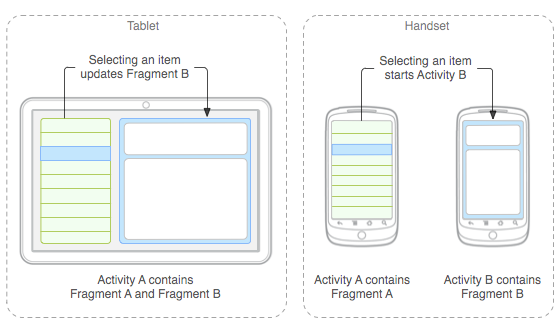
\includegraphics[scale=0.60]{img/fragments_modules}
\caption{Beispiel man kann mithilfe von Fragments Views erstellen, die sowohl auf einem Tablet als auch auf einem Handy ein optimales Benutzerinterface anbieten}
\end{figure}

\newpage
\subsection{Der Lifecycle}
Ein Fragment ist immer eingebunden in eine Activity und ist direkt vom Lifecycle der übergeordneten Activity abhängig.
Wird die übergeordnete Activity pausiert oder zerstört werden auch alle untergeordneten Fragments pausiert oder zerstört.
Das Aufbauen der Benutzeransicht erfolgt in der onCreateView() Methode.

\ \\
\texttt{In einem Fragment:}
\begin{lstlisting}
@Override
public View onCreateView(LayoutInflater inflater, ViewGroup container, Bundle savedInstanceState) {
        super.onCreate(savedInstanceState);
        return inflater.inflate(R.layout.example_fragment, container, false);
    }
\end{lstlisting}


\subsection{Fragment Transactions}
Mittels Transaktionen lassen sich Fragments hinzufügen, entfernen oder ersetzen.
Es werden mehrere dieser Aktionen hintereinander abgesetzt und zusammen nach einem commit() ausgeführt.
Ein Fragment kann mittels addToBackStack() auch zum BackStack hinzugefügt werden um dadurch, ähnlich wie bei Activites, Navigation mit dem BackButton zu ermöglichen.
Dabei ist zu beachten, dass alle Aktionen vor einem commit() gemeinsam auf den BackStack gelegt werden und bei drücken des BackButtons alle gemeinsam aufgehoben werden.
Wird addToBackStack() nicht aufgerufen, wird ein Fragment beim Schließen oder beim Wechseln auf ein anderes Fragment zerstört und kann nicht mehr aufgerufen werden.

\begin{lstlisting}
        FragmentManager fragmentManager = getFragmentManager();
        FragmentTransaction fragmentTransaction = fragmentManager.beginTransaction();
        fragmentTransaction.addToBackStack(null);
        fragmentTransaction.replace(R.id.fraPlace, fragment);
        fragmentTransaction.commit();
\end{lstlisting}

\newpage
\subsection{Verwendung von Fragments}
In dieser Arbeit werden Fragments verwendet, um die Benutzeransichten, ausgenommen des NavigationDrawers, anzuzeigen.
Dabei wird ein FrameLayout im Layoutfile der MainActivity durch ein Fragment mittels der displayView() Methode ersetzt.
Navigation durch diese Fragments wird mittels den Buttons im MFragment oder dem NavigationDrawer ermöglicht.

\ \\
\texttt{MainActivity.java und MFragment.java:}
\begin{lstlisting}
private void displayView(Fragment fragment) {
        FragmentManager fragmentManager = getFragmentManager();
        FragmentTransaction fragmentTransaction = fragmentManager.beginTransaction();
        fragmentTransaction.addToBackStack(null);
        fragmentTransaction.replace(R.id.fraPlace, fragment);
        fragmentTransaction.commit();
    }
\end{lstlisting}

\ \\
\texttt{activity\_main.xml:}
\begin{lstlisting}
<FrameLayout
        android:id="@+id/fraPlace"
        android:layout_width="match_parent"
        android:layout_height="match_parent" />
\end{lstlisting}

\begin{figure}
	\begin{subfigure}[b]{0.3\textwidth}
	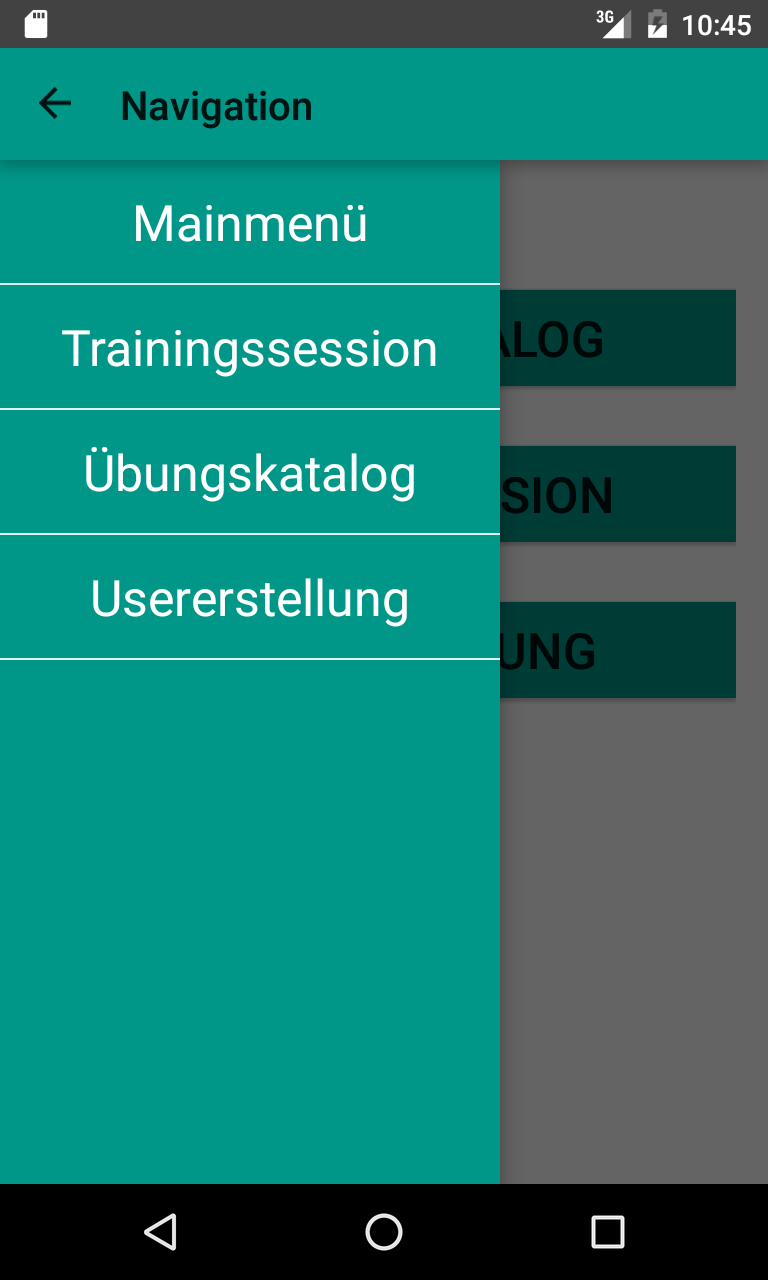
\includegraphics[scale=0.20]{img/NavigationDrawer}
	\end{subfigure}
	\hfil
	\begin{subfigure}[b]{0.3\textwidth}
	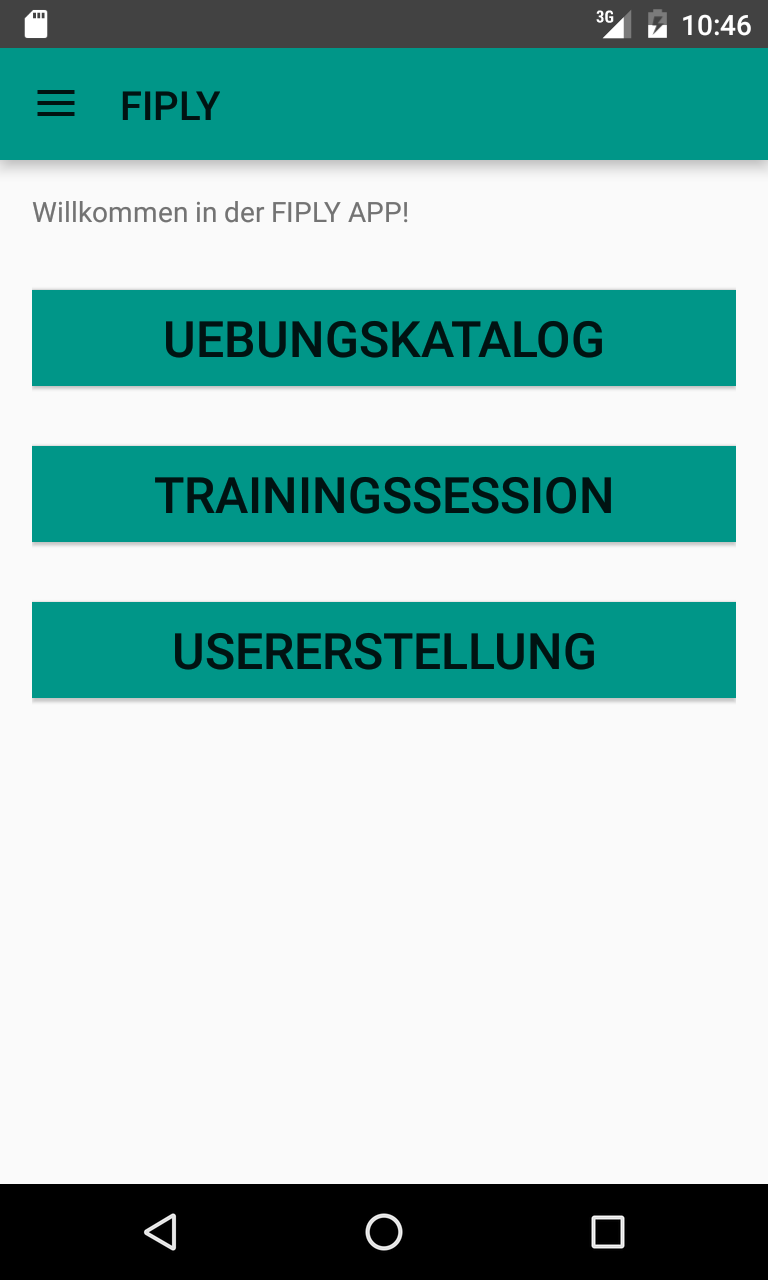
\includegraphics[scale=0.20]{img/MFragment}
	\end{subfigure}	
	\caption{Bild des NavigationDrawers und des FMains}
\end{figure}


\begin{figure}
	\begin{subfigure}[b]{0.3\textwidth}
	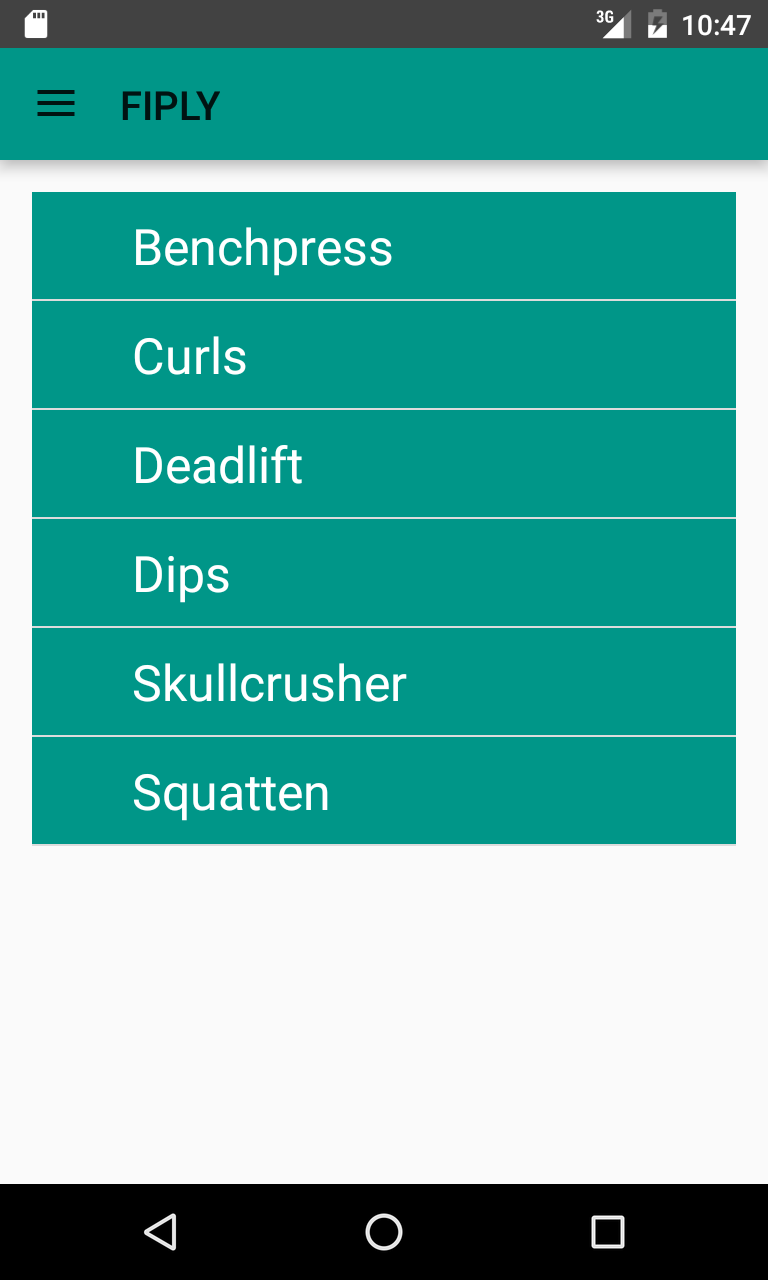
\includegraphics[scale=0.20]{img/Uebungskatalog}
	\end{subfigure}
	\hfil
	\begin{subfigure}[b]{0.3\textwidth}
	
\includegraphics[scale=0.20]{img/Uebungskatalog_detail_video}
	\end{subfigure}	
	\caption{Bei Klicken eines Elements in der ListView wird die zugehörige DetailView aufgerufen}
\end{figure}


\end{document}
